% !TEX root = ../lab2_report.tex
% ═══════════════════════════════════════════════════════════════
% 实验四：平面叶栅叶片表面压力分布测量
% ═══════════════════════════════════════════════════════════════

\section{实验四：平面叶栅叶片表面压力分布测量}

\subsection{实验目的}

\begin{enumerate}
    \item 熟悉平面叶栅实验设备和实验方法。
    \item 掌握叶片表面静压分布和等熵马赫数分布的测量与计算方法。
    \item 绘制叶片表面压力分布曲线和等熵马赫数分布曲线。
    \item 了解平面叶栅实验在压气机气动设计中的作用和地位。
\end{enumerate}

\subsection{实验原理}

叶片表面马赫数分布是评估叶栅气动性能的重要依据。气流流经压气机叶栅时，在吸力面（叶背）加速形成低压区，在压力面（叶盆）减速形成高压区，吸力面和压力面的静压差构成叶片的气动负荷。通过分布在叶片表面不同弦向位置的静压孔测得静压分布，可以计算静压系数 $C_p$ 和基于等熵假设的当地马赫数 $Ma$，从而评估叶型的载荷分布特征和扩压能力。

\subsection{实验装置}

\subsubsection{叶栅风洞}

由离心压气机连续供气，气流经扩压段减速扩压后进入稳定箱（内装蜂窝器和阻尼网消除来流旋涡），再经收敛段加速后进入叶栅试验段。试验段可绕中心转动以改变叶栅来流攻角。

\subsubsection{叶栅参数}

试验叶栅采用 NACA-65 叶型，主要几何参数见表~\ref{tab:cascade_params}。

\begin{table}[H]
\centering
\caption{NACA-65 叶栅几何参数}
\label{tab:cascade_params}
\begin{tabular}{ll}
\toprule
参数 & 数值 \\
\midrule
叶片数 & 6 \\
叶片安装角 $\beta_s$ & 68\textdegree \\
叶片弦长 $b$ & 52 mm \\
叶片弯角 $\theta$ & 54\textdegree \\
进口几何角 $\beta_{1k}$ & 35.6\textdegree \\
出口几何角 $\beta_{2k}$ & 85.6\textdegree \\
栅距 $t$ & 32.5 mm \\
相对栅距 $\bar{t} = t/b$ & 0.625 \\
\bottomrule
\end{tabular}
\end{table}

\subsubsection{角度关系}

进口气流角与转盘刻度的关系：
\begin{equation}
    \beta_1 = 25\textdegree + \gamma
\end{equation}

式中 $\gamma$ 为转盘刻度。攻角定义为气流方向与叶型中弧线前缘切线的夹角：
\begin{equation}
    i = \beta_1 - 35.6\textdegree
\end{equation}

当 $\gamma = 10.6\textdegree$ 时，$\beta_1 = 35.6\textdegree$，对应 $i = 0\textdegree$（零攻角）。

静压测点布置于叶片吸力面（6个）和压力面（6个），沿弦向位置为 $x/b = 1/7, 2/7, \dots, 6/7$。

\subsection{实验步骤}

\begin{enumerate}
    \item 转动转盘将叶栅调至目标攻角（0\textdegree~攻角对应转盘刻度 $10.6\textdegree$）。
    \item 记录实验室大气温度 $T_{\text{atm}}$ 和大气压力 $P_{\text{atm}}$。
    \item 启动离心风机，变频器调至50 Hz。
    \item 读数稳定后，记录进口总压 $P_1^*$（由进口总压探针测量）和进口静压 $P_1$。
    \item 依次读取并记录叶片吸力面和压力面共12个测点的静压值。
    \item 改变攻角至 $-5\textdegree$（转盘刻度 $5.6\textdegree$）和 $+5\textdegree$（转盘刻度 $15.6\textdegree$），重复步骤\textbf{4-5}。
    \item 实验结束：关闭风机，整理设备。
\end{enumerate}

\subsection{数据处理方法}

\subsubsection{静压系数}

\begin{equation}
    C_p = \frac{P - P_1}{P_1^* - P_1}
\end{equation}

式中 $P$ 为叶片表面某测点的静压，$P_1$ 为进口截面静压，$P_1^*$ 为进口截面总压。静压系数的取值范围通常为 $C_p \in [-1, 1]$。

\subsubsection{等熵马赫数（不可压缩假设）}

当地速度由伯努利方程计算：
\begin{equation}
    v_i = \sqrt{\frac{2(P_1^* - P_i)}{\rho}}
\end{equation}

空气密度：
\begin{equation}
    \rho = \frac{P_{\text{atm}}}{R \cdot T_{\text{atm}}}, \quad R = 287.058\ \text{J/(kg·K)}
\end{equation}

当地马赫数：
\begin{equation}
    Ma_i = \frac{v_i}{a}, \quad a = \sqrt{\gamma R T_{\text{atm}}}, \quad \gamma = 1.4
\end{equation}

\subsection{数据处理结果及分析}

\subsubsection{静压系数分布}

\begin{figure}[H]
    \centering
    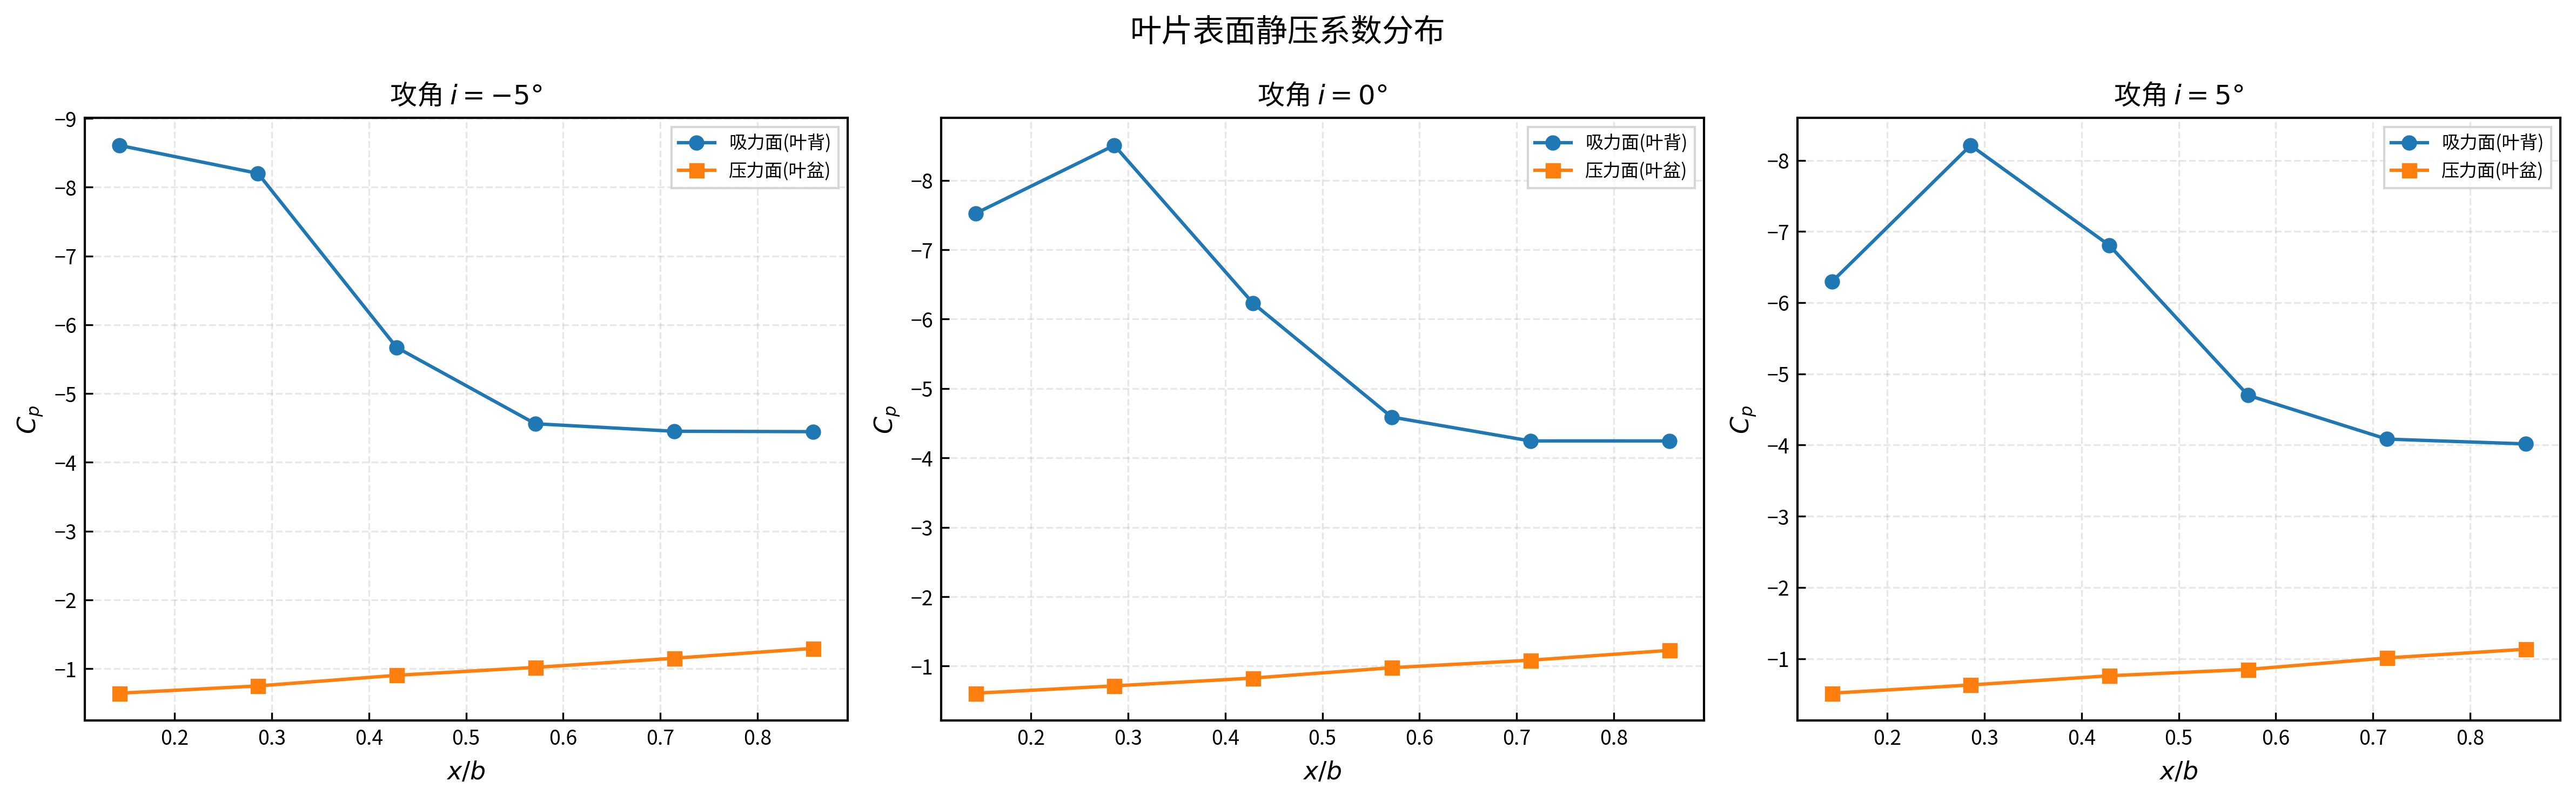
\includegraphics[width=\textwidth]{figures/exp4_cp_distribution.png}
    \caption{叶片表面静压系数分布（-5\textdegree, 0\textdegree, +5\textdegree~攻角）}
    \label{fig:cp}
\end{figure}

图~\ref{fig:cp} 展示了三个攻角下吸力面和压力面沿弦向的 $C_p$ 分布。可以看出：
\begin{enumerate}
    \item 吸力面 $C_p$ 为负值（相对于进口静压为低压），压力面 $C_p$ 为正值（高压），两者之差构成叶片的气动负荷。
    \item 吸力面前缘（$x/b = 1/7$）附近 $C_p$ 出现最低值（吸力峰），气流在此处达到最大加速。
    \item 从 $x/b = 2/7$ 开始，吸力面 $C_p$ 逐渐回升（逆压梯度），气流减速扩压。
    \item 不同攻角下 $C_p$ 分布形态相似，但正攻角时吸力面和压力面的压差增大（负荷增大），负攻角时压差减小。
\end{enumerate}

\subsubsection{等熵马赫数分布}

\begin{figure}[H]
    \centering
    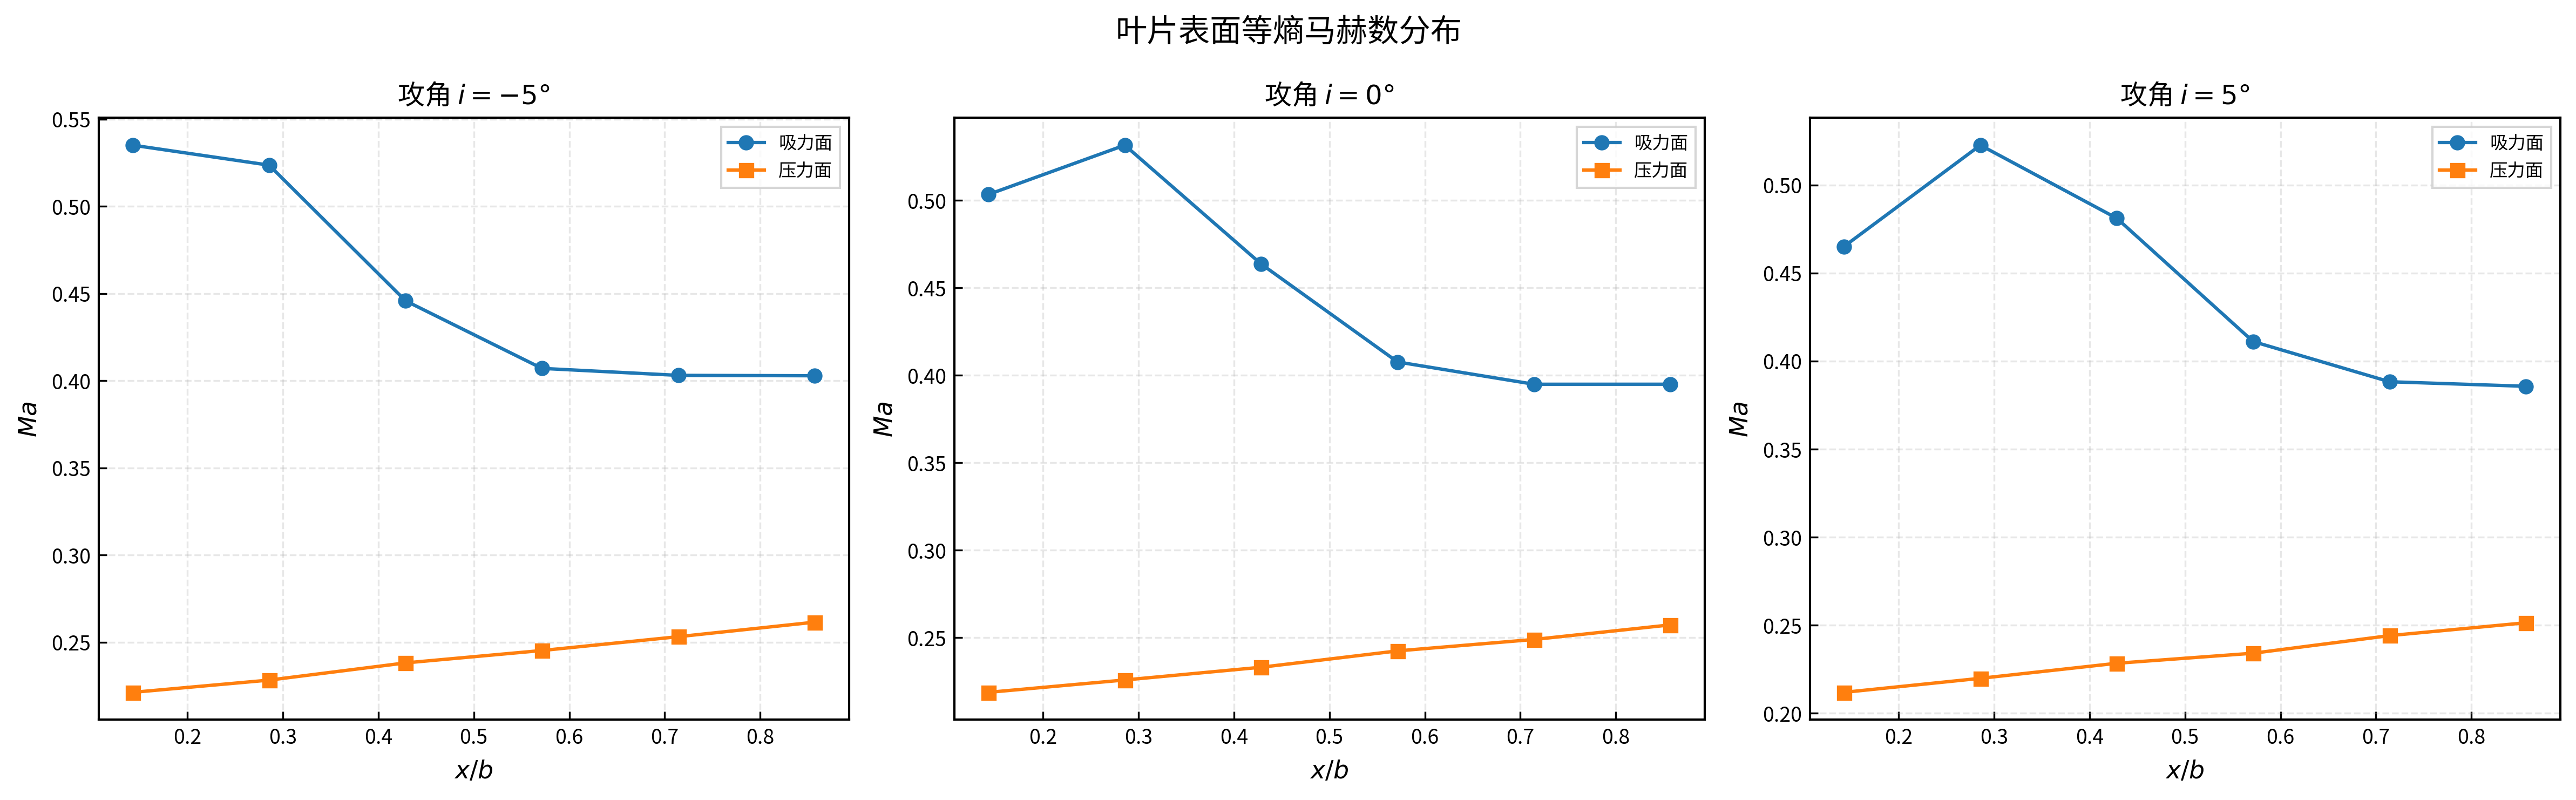
\includegraphics[width=\textwidth]{figures/exp4_mach_distribution.png}
    \caption{叶片表面等熵马赫数分布（-5\textdegree, 0\textdegree, +5\textdegree~攻角）}
    \label{fig:mach}
\end{figure}

图~\ref{fig:mach} 展示了三个攻角下吸力面和压力面沿弦向的 $Ma$ 分布。可以看出：
\begin{enumerate}
    \item 吸力面马赫数沿弦向先增大后减小，在前缘附近出现吸力峰（最大马赫数），反映气流在叶片前缘的强烈加速过程。
    \item 压力面马赫数沿弦向单调下降，气流持续减速扩压。
    \item 正攻角时吸力峰更突出（Ma更高），说明前缘附近的气流加速更强，但也意味着更大的逆压梯度（下游减速更剧烈），附面层分离的风险增大。
    \item 负攻角时压力面和吸力面的马赫数差值减小，叶片气动负荷降低。
\end{enumerate}

\subsubsection{结果讨论}

\begin{enumerate}
    \item \textbf{载荷分布特征}：NACA-65 叶型属于典型的压气机控制扩散叶型，其吸力面马赫数分布呈"前加载"特征——最大马赫数出现在前缘附近，之后逐步减速扩压，避免在吸力面出现强激波（跨音速时）或强逆压梯度导致的分离。
    \item \textbf{攻角影响}：增大攻角使叶片负荷增大（吸力面-压力面压差增大），但也使吸力面逆压梯度增强，超过临界攻角时可能导致附面层分离和性能急剧恶化。
    \item \textbf{设计意义}：叶片表面压力分布实验是叶型设计和优化的基本手段，通过调整叶型中弧线和厚度分布可以控制表面马赫数分布，达到扩压能力与损失之间的最优折中。
\end{enumerate}

\subsection{结论}

通过平面叶栅叶片表面压力分布测量，成功获取了NACA-65叶型在 $-5\textdegree$、$0\textdegree$、$+5\textdegree$ 三个攻角下的静压系数和等熵马赫数分布。吸力面前缘的吸力峰特征和后部的逆压梯度分布符合典型压气机叶型的流动规律。攻角增大使叶片负荷增大但逆压梯度增强，印证了叶栅气动设计中"负荷-损失"折中的基本理念。
